\section{Introduzione alla teoria dell'utilità e decision making}
\subsection{Concetti di base}
\subsubsection{ALTERNATIVE}
Parliamo di \textit{agenti} che devono scegliere un'\textit{alternativa} da
un'insieme $\mathcal{X}$ di alternative. Questo insieme di alternative ha degli
elementi che possono essere \textbf{esaustivi} o \textbf{mutualmente
    esclusivi}.

\textbf{Esepmio}: $\mathcal{x}$ \{
\begin{itemize}
    \item DL = Deep Learning
    \item AGT = Algorithmic Game Theory
    \item DLAGT = Deep Learning Algorithmic Game Theory
    \item N = None
\end{itemize}
\}

\subsubsection{PREFERENZE}

Con il termine \textbf{preferenze} identifichiamo una relazione $\succcurlyeq$
su $\mathcal{X}$, che è un sottoinsieme di $\mathcal{X} \times \mathcal{X}$. Le
preferenze possono essere:
\begin{itemize}
    \item \textbf{complete} se $\forall x,y \in \mathcal{X}$ vale $x \succcurlyeq y$ oppure $y \succcurlyeq x$
    \item \textbf{transitive} se $\forall x,y,z \in \mathcal{X}$ vale $x \succcurlyeq y$ e $y \succcurlyeq z$ allora $x \succcurlyeq z$
\end{itemize}

\subsubsection{Relazione di Preferenza}

Una preferenze è una \textbf{relazione di preferenza} se è sia
\textbf{completa} che \textbf{transitiva}.

Si chiama preferenza \textbf{stretta} se $x \succ y \iff x \succcurlyeq y$ e $x
    \nsucceq y$.

Si chiama \textbf{indifferenza} se $x \sim y \iff x \succcurlyeq y$ e $x
    \preccurlyeq y$.

\subsubsection{Rappresentare le preferenze come \textbf{utilità}}

Una relazione di preferenza puà essere tradotta in una funzione di utilità del
tipo $u: \mathcal{X} \rightarrow \mathbb{R}$. Si può fare in questo modo:

\begin{equation}
    x \succcurlyeq y \iff u(x) \geq u(y) \quad \forall x,y \in \mathcal{X}
\end{equation}

\textit{Esempio:} Se un agente dovesse trovare \textit{x} almeno buono quanto \textit{y}, allora la funzione di utilità $u(x)$ deve essere almeno
alta quanto $u(y)$. Cioè l'agente è come se stesse \textbf{massimizzando} il valore di $u(var)$.

\begin{theorem}[Rappresentazione Ordinale]

    Sia $\mathcal{X}$ un insieme finito di alternative e sia $\succcurlyeq$ una
    relazione di preferenza su $\mathcal{X}$. Allora una preferenza può essere
    rappresentata come una funzione di utilità $u: \mathcal{X} \rightarrow
        \mathbb{R}$ se e solo se è \textbf{completa} e \textbf{transitiva}. In più, se
    $f:\mathcal{R} \rightarrow \mathcal{R}$ è una funzione monotona crescente,
    allora $f \circ u$ rappresenta la stessa preferenza di $u \succcurlyeq$

    \textbf{Nota}: dall'ultimo statement, l'ordine ha rilevanza.

    Per essere valido ci sono 2 condizioni necessarie:
    \begin{itemize}
        \item Transitività: Cioè, dato $\mathcal{X} = \{a,b,c\}$, suponiamo che $a \succ b
                  \succ c \succ a \implies u(a) > u(b) > u(c) > u(a)$. Questo sarebbe
              \textbf{assurdo}.
        \item Completezza: Se abbiamo preferenze incomplete, allora al massimo possiamo
              costruire un ordine per un sottoinsieme di $\mathcal{X}$.
    \end{itemize}
\end{theorem}

\begin{dimostrazione}[Rappresentazione Ordinale]
\end{dimostrazione}

La transitività e la completezza sono necessarie e sufficienti. Supponiamo di
avere l'insieme $X = \{X_1, \ldots, X_n\}$. Possiamo suddividere gli elementi
di $X$ in $k$ classi di indifferenza $C_1, \ldots, C_k$ tali che $C_1 \succ C_2
    \succ \ldots \succ C_k$. In questo modo, possiamo definire la funzione di
utilità $u$ in modo che:

\[
    u(x) = k \quad \forall x \in C_1,
\]
\[
    u(x) = k-1 \quad \forall x \in C_2,
\]
\[
    \ldots
\]
\[
    u(x) = 1 \quad \forall x \in C_k.
\]

In questo contesto, $\succ$ rappresenta la relazione di preferenza.

\subsection{Le lotterie}

Una lotteria è una tupla $\mathcal{L} = (p_1,x_1;p_2,x_2 \ldots, p_n,x_n)$.

\begin{itemize}
    \item Con prezzo monetario $x_1,x_2, \dots, x_n \in X \subseteq R$.
    \item Distribuzione di probabilità $(p_1, p_2, \dots, p_n)$.
\end{itemize}

Quindi con $\mathcal{L}$ viene definito l'insieme delle lotterie semplici.

Un esempio di lotteria è il seguente:
\[
    L = (0.3,10; 0.2,5; 0.1,0; 0.4,-5)\]
Possiamo calcolare il valore atteso per la lotteria come:
\[
    \mathbb{E}(L) = \sum_{i=1}^n {p_i}{x_i}
\]
\[
    \mathbb{E} = 0.3 \times 10 + 0.2 \times 5 + 0.1 \times 0 + 0.4 \times (-5) = 2
\]

\begin{definition}[Utilità attesa]
    Data una relazione di preferenza $\succcurlyeq$ su $\mathcal{L}$, una funzione di utilità $U: \mathcal{L} \rightarrow \mathbb{R}$ è
    funzione di utilità attesa se può ssere scritta come:
\end{definition}

\[
    U(L) = \sum_{i=1}^n{p_i}u(x_i)
\]
dove $p_i$ è la probabilità che l'evento $x_i$ accada e u è la funzione di
utilità di Bernoulli.

per un qualche funzione $u:R \rightarrow R$.

Questa funzione $u$ viene chiamata \textbf{funzione di utilità di Bernoulli}

\subsection{Utilità di Von Neumann-Morgenstern}

I due matematici Von Neumann e Morgenstern hanno dimostrato che se una
relazione di preferenza $\succcurlyeq$ su $\mathcal{L}$ soddisfa le seguenti
proprietà, allora può essere rappresentata come una funzione di utilità:
\begin{itemize}
    \item \textbf{Assioma 1} (Ordine di preferenza): $\succcurlyeq$ è \textbf{completa} e \textbf{transitiva}
    \item \textbf{Assioma 2} (Continuità): Se $L \succ M \succ N$ allora esiste $p \in [0,1]$ tale che $pL + (1-p)N \sim M$
    \item \textbf{Assioma 3} ( Indipendenza): Per una qualsiasi lotteria $N$ e $p \in [0,1], L \succcurlyeq M \iff pL + (1-p)N \succcurlyeq pM + (1-p)N$
\end{itemize}

\begin{theorem}[Teorema di VNM]
    Una relazione binaria $\succ$ su $\mathcal{L}$ ha una rappresentazione utilità attesa se e solo se soddisfa gli assiomi da 1 a 3. Ancora, se $U$ e $V$ sono
    rappresentazioni di utilità attesa di $\succ$, allora esistono delle costanti $a,b \in \mathbb{R}$ tale che $U(\cdot) = aV(\cdot)+b$.
\end{theorem}

Che detto in parole italiane, significa che se una relazione binaria è
completa, transitiva, continua e indipendente, allora può essere rappresentata
come una funzione di utilità attesa.

Andremo a fare la \textbf{dimostrazione} in due fasi:
\begin{enumerate}
    \item Dimostriamo che $U(L) \sum_{i=1}^n p_i u(x_i)$
    \item Dimostriamo che $L \succ M \iff U(L) \succ U(M)$ con $L,M \in \mathcal{L}$
\end{enumerate}

\begin{dimostrazione}[Parte 1 VNM]
\end{dimostrazione}
Supponiamo di avere $n$ risultati $o_1, \dots, o_n$.

Per la \textbf{completezza} e per la \textbf{transitività} possiamo ordinare i
nostri risultati dal peggiore al migliorare
\[
    o_1 \curlyeqprec \dots \curlyeqprec o_n
\]
Sia $u(0_1) = 0$ e $u(o_n) = 1$.

Per ogni provabilità $p \in [0,1]$, definiamo una lotteria $\mathcal{L}(p) = p
    \cdot o_n + (1-p) \cdot o_1$.

Per l'assioma di continuità c'è una probabilità $q_1 \in [0,1]$, per ogni
risultati, tale che $L(q_i) = o_i$ e $u(o_i) = q_i$

Segue che l'utilità della lotteria $\mathbb{M} = \sum_i p_i o_i$ è il valore
atteso di $u$.

\[
    u(M) = u(\sum_i p_i o_i) = \sum_i p_i u(o_i) = \sum_i p_i q_i
\]

\begin{dimostrazione}[Parte 2 VNM]
\end{dimostrazione}

Supponiamo che $L `succ M$, possiamo definire $L'$ e $M'$ come segue:
\[
    \begin{aligned}
        L' = U(L) \cdot o_n + (1-U(L)) \cdot o_1 \\
        M' = U(M) \cdot o_n + (1-U(M)) \cdot o_1
    \end{aligned}
\]

Abbiamo il seguente ordine: $\mathcal{L}' \sim L \succ M \sim M'$.

Poiché $L' \succ M' \implies U(L) > U(M)$.

Questo implica $ L \succ M \iff U(L) > U(M)$.

\subsection{Atteggiamento verso il rischio}C

Consideriamo una lotteria giusta $\mathcal{L} = p \cdot x + (1-p) \cdot y = 0$

Allora:

\begin{itemize}
    \item Un giocatore è \textbf{neutrale al rischio} $\iff$ la sua funzione di utilità è
          \textbf{lineare}. Cioè: $u(x) = ax + b$. \textit{Si dice che un giocatore
              neutrale al rischio sia neutrale con le lotterie giuste }
    \item Un giocatore è \textbf{avverso al rischoi} $\iff$ la sua funzione di utilità è
          \textbf{concava}. \textit{Un giocatore avverso al rischio non gioca a nesusuna
              lotteria giuste}
    \item Un giocatore è \textbf{propenso al rischio} $\iff$ la sua funzione di utilità è
          \textbf{convessa}. \textit{Un giocatore propenso al rischio gioca a tutte le
              lotterie giuste}
\end{itemize}

\begin{figure}[H]
    \centering
    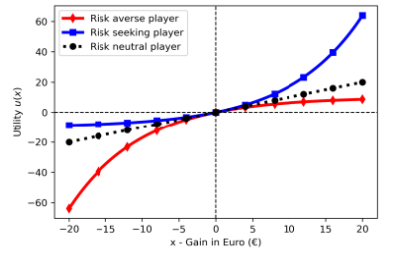
\includegraphics[scale=0.7]{chapters/images/rishio.png}
    \caption{Rappresentazione grafica del rischio}
    \label{fig:rischio}
\end{figure}

\subsection{Applicazioni: Condivisione del rischio}

Immaginiamo di avere due giocatori $A$ e $B$ che sono \textit{avversi al
    rischio} con

$u(x) = \sqrt(x)$ e due \textit{assets} $A_1, A_2 = (0.5, 100; 0.5, 0)$. Supponiamo che $A_1$ e $A_2$ siano indipendenti.

L'utilità di $A_1$ e $A_2$ è : $u(A_1) 0 u(A_2) = 0.5 \times \sqrt(100) = 5$

Se i due giocatori formassero un \textbf{fondo comune} dove ogni giocatore ha
una quota della metà, ogni giocatore ha l'asset $A_m = (0.25, 100; 0.5, 50;
    0.25, 0)$.

L'utilità di un gioatore è:

\[
    u(A_m) = 0.25 \times \sqrt(100) + 0.5 \times \sqrt(50) \thickapprox 6.
\]

Questo perché il giocatore ha una probabilità del 50\% di avere 100 e una
probabilità del 50\% di avere 50. Quindi la media è 75 e la radice è 6.

\subsection{Applicazione: Assicurazione}

Supponiamo di avere un giocatore $A$ che è \textit{avverso al rischio} con
$u(x) = \sqrt(x)$ e un asset $A = (0.5, 100; 0.5, 0)$.

Immaginiamo di avere una compagnia di assicurazione neutrale al rischio con
tantissimi soldoni.

Quale premium $P$ pagherebbe il giocatore per assicurare il suo asset?

\[\
    u(100-P) \geq 0.5 \times u(100) + 0.5 \times u(0) \rightarrow \sqrt(100-P) \geq 5 \rightarrow 100-P \geq 25 \rightarrow -P \geq -100+25 \rightarrow P \geq 75
\]

Quale premium pagherebbe la compagnia assicurativa per assicurarsi l'asset del
giocatore?

\[
    P \geq 0.5 \times 100 + 0.5 \times 0 \rightarrow P \geq 50
\]

Allora, entrambi guadagnerebbero soldi se la compagnia assicurasse l'asset del
player per un premium $P \in [50,75]$.

\newpage